% Activate the following line by filling in the right side. If for example the name of the root file is Main.tex, write
% "...root = Main.tex" if the chapter file is in the same directory, and "...root = ../Main.tex" if the chapter is in a subdirectory.
 
%!TEX root =  

\chapter{Templates}

\subsection{Status Reports}
\begin{figure}[htbp]
\begin{center}
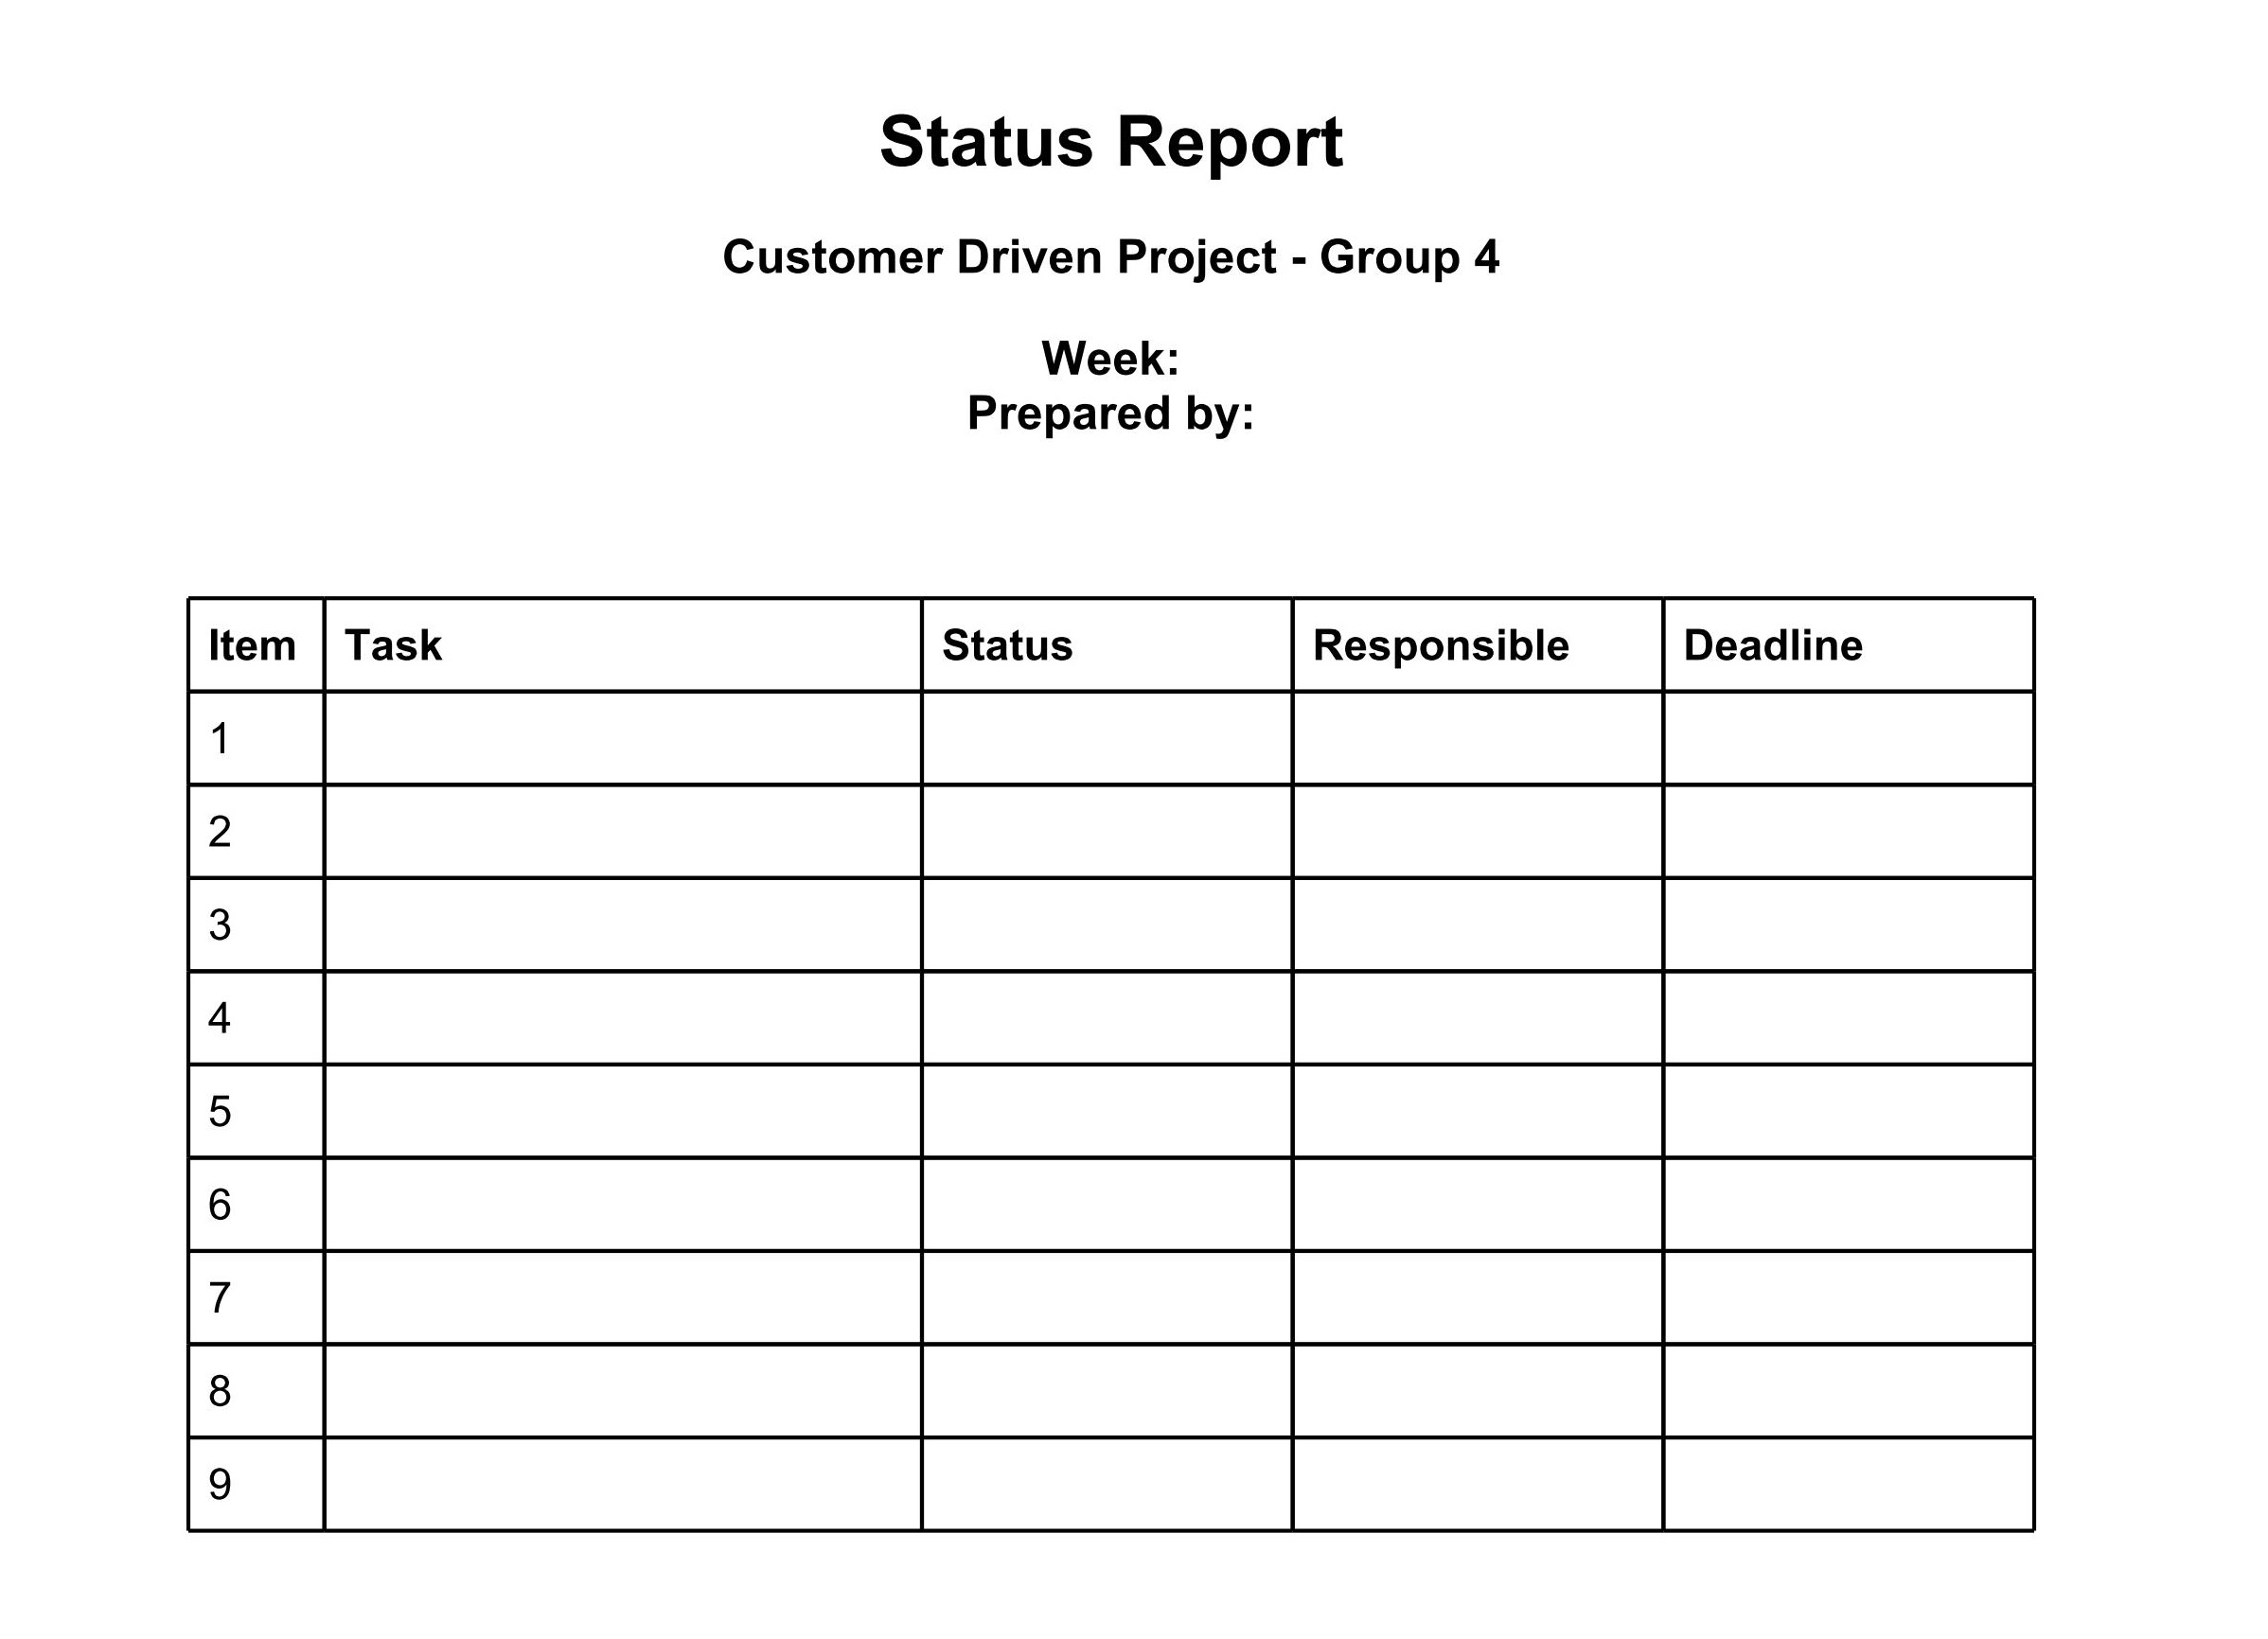
\includegraphics[width = \textwidth]{Appendix/statusreportTemp.jpg}
\caption{Status Report Template.}
\label{StatusReportTemplate}
\end{center}
\end{figure}

\subsection{Meeting Notes}
\begin{figure}[hbp]
\begin{center}
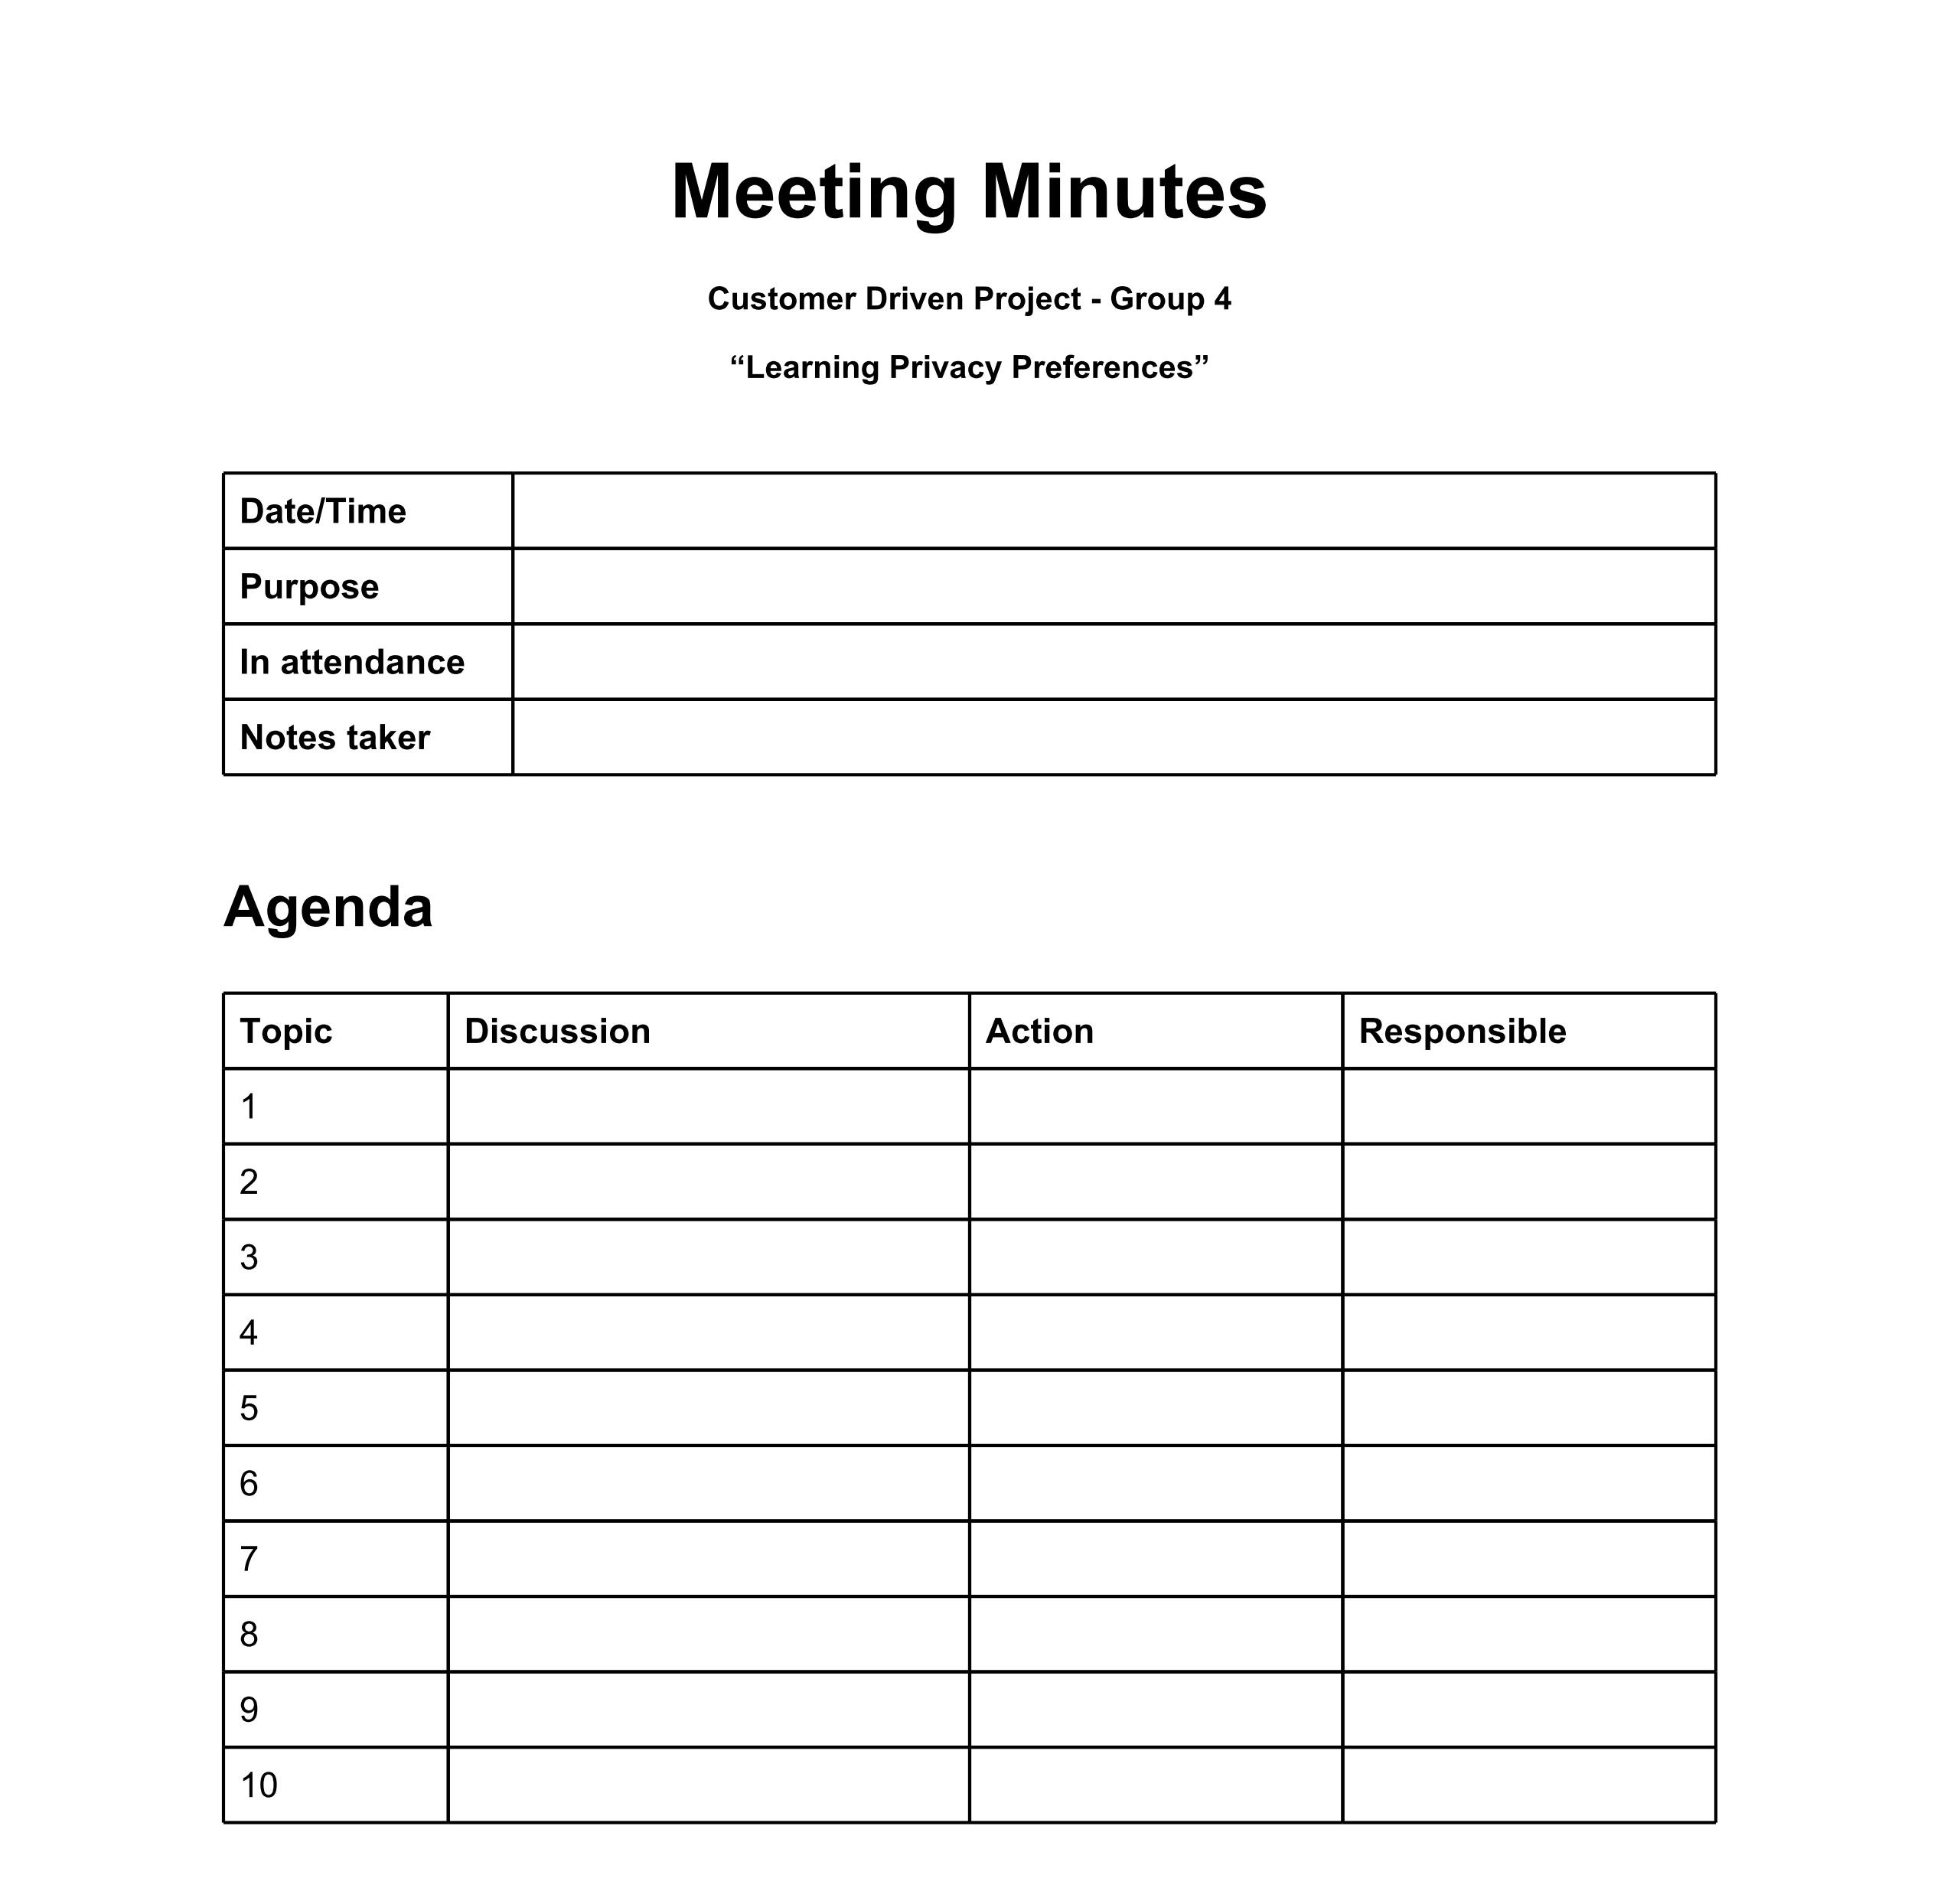
\includegraphics[width = \textwidth/3*2]{Appendix/meetingreportTemp.jpg}
\caption{Meeting Report Template.}
\label{MeetingReportTemplate}
\end{center}
\end{figure}
\newpage

\subsection{Time Reporting}
\begin{figure}[hbp]
\begin{center}
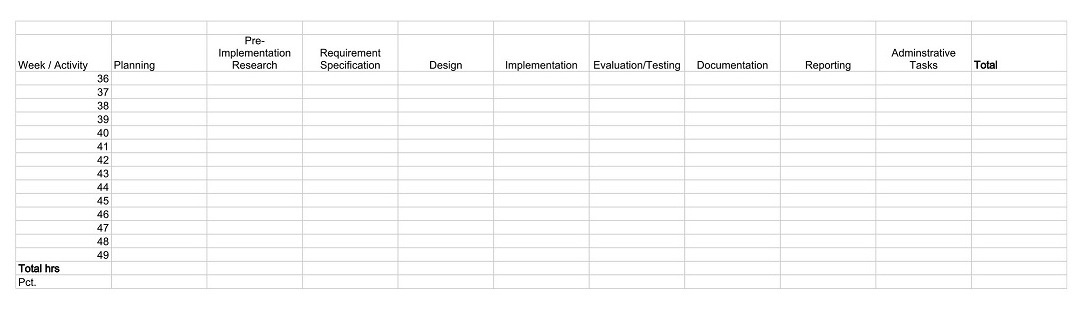
\includegraphics[width = \textwidth]{Appendix/timereportTemp.jpg}
\caption{Time Report Template.}
\label{TimeReportTemplate}
\end{center}
\end{figure}

\subsection{Test Plan}
\begin{figure}[hthp]
\begin{center}
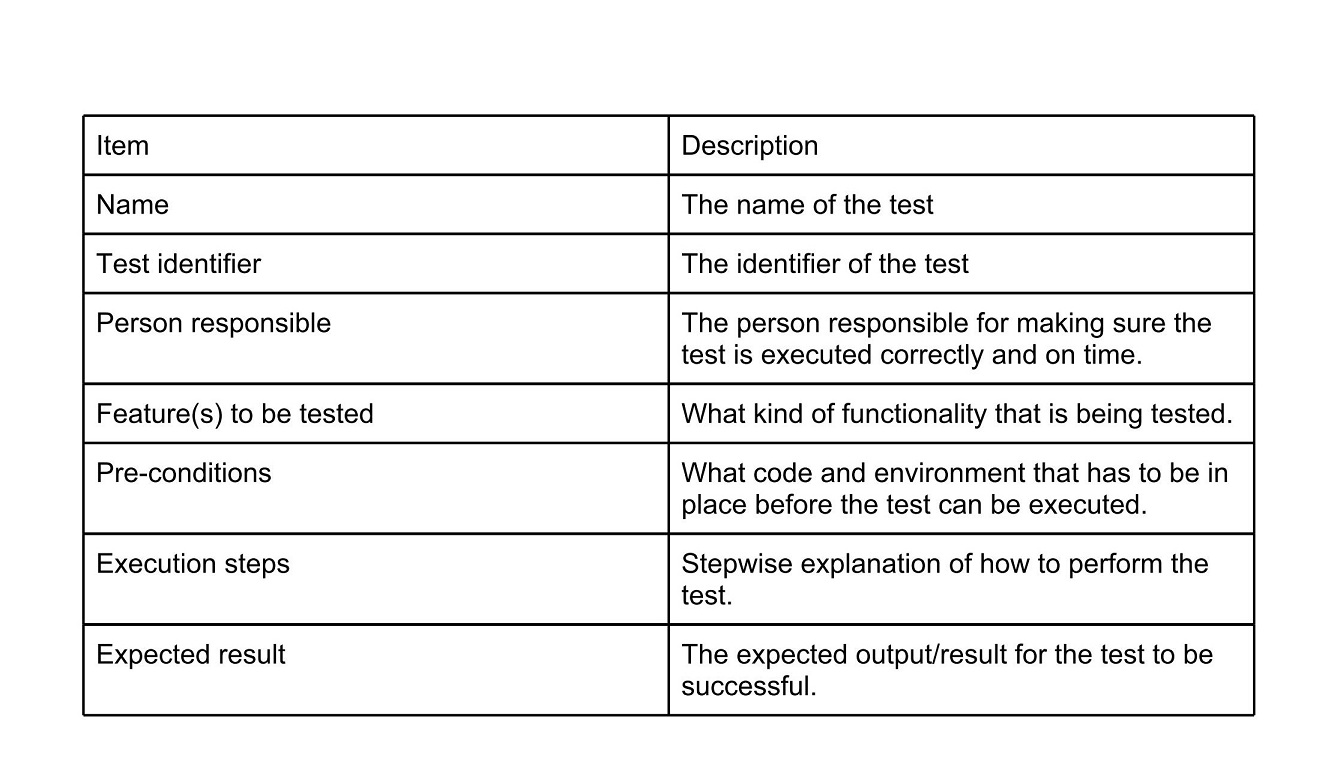
\includegraphics[width = \textwidth/3*2]{Appendix/testplanTemp.jpg}
\caption{Test Plan Template.}
\label{TestPlanTemplate}
\end{center}
\end{figure}
\newpage

\subsection{Java documentation}
\begin{figure}[hthp]
\begin{center}
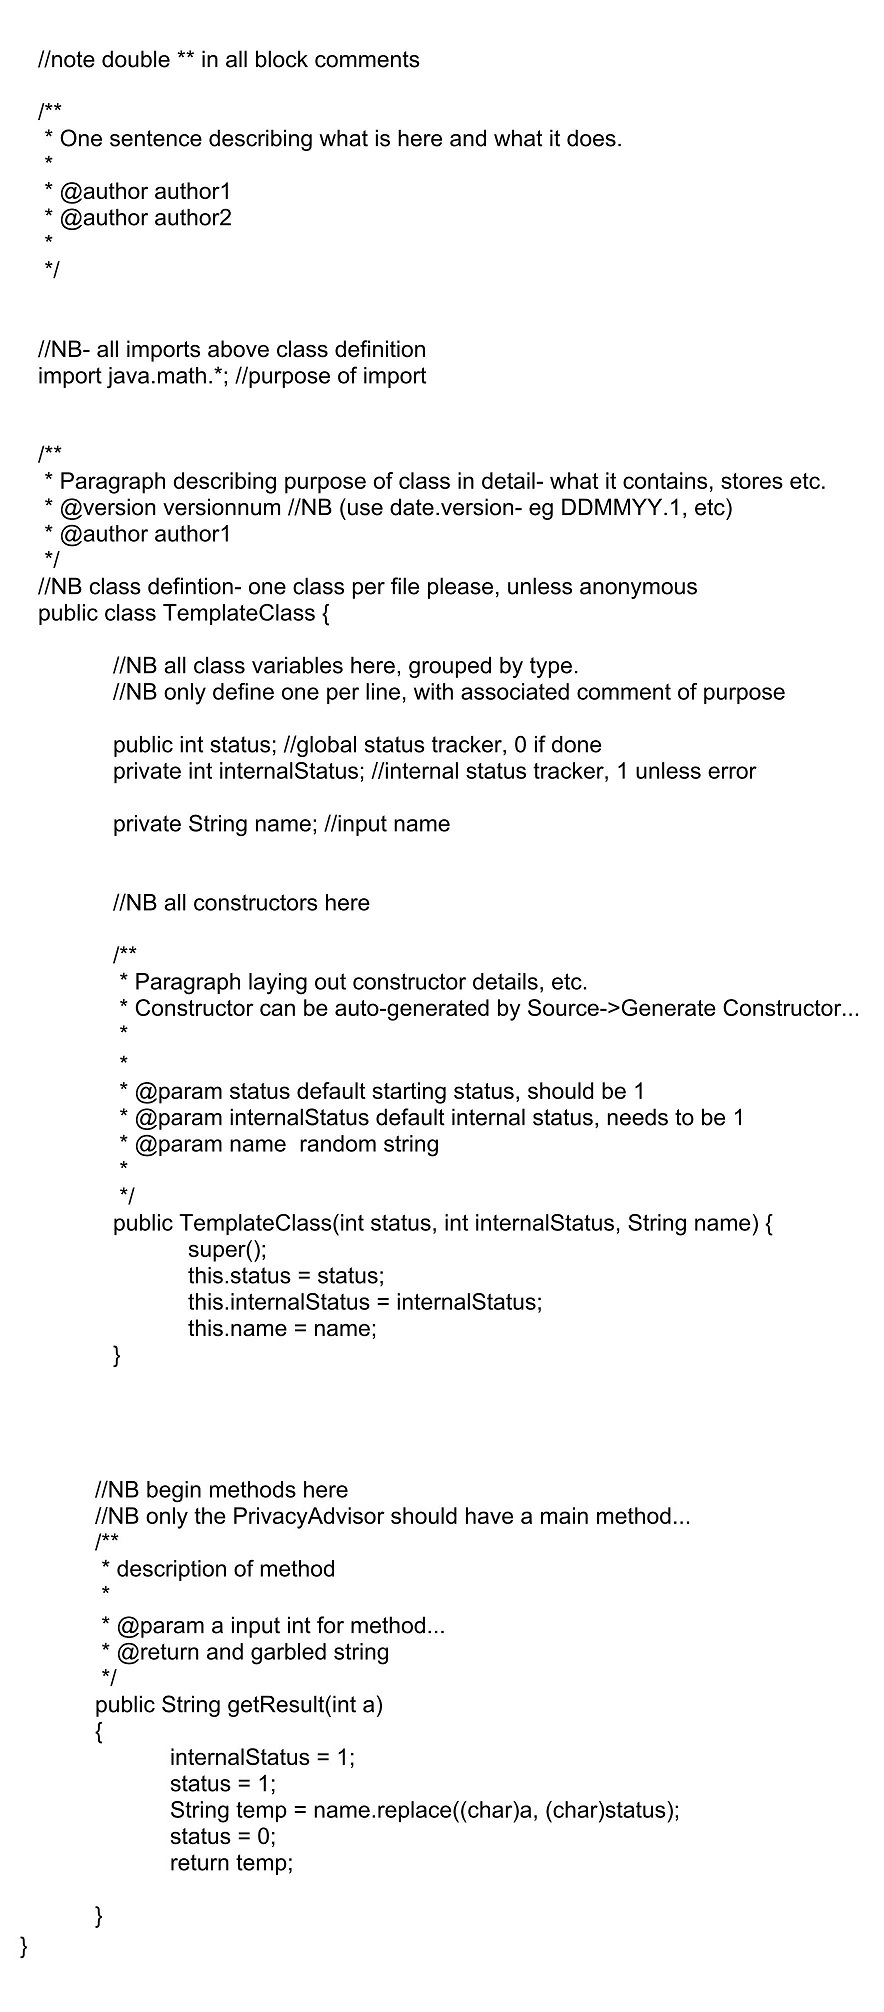
\includegraphics[height = \textheight/3*2]{Appendix/javadocTemp.jpg}
\caption{Javadoc Template.}
\label{JavadocTemplate}
\end{center}
\end{figure}
